\makeatletter
\tikzset{
    database/.style={
        path picture={
            \draw (0, 1.5*\database@segmentheight) circle [x radius=\database@radius,y radius=\database@aspectratio*\database@radius];
            \draw (-\database@radius, 0.5*\database@segmentheight) arc [start angle=180,end angle=360,x radius=\database@radius, y radius=\database@aspectratio*\database@radius];
            \draw (-\database@radius,-0.5*\database@segmentheight) arc [start angle=180,end angle=360,x radius=\database@radius, y radius=\database@aspectratio*\database@radius];
            \draw (-\database@radius,1.5*\database@segmentheight) -- ++(0,-3*\database@segmentheight) arc [start angle=180,end angle=360,x radius=\database@radius, y radius=\database@aspectratio*\database@radius] -- ++(0,3*\database@segmentheight);
        },
        minimum width=2*\database@radius + \pgflinewidth,
        minimum height=3*\database@segmentheight + 2*\database@aspectratio*\database@radius + \pgflinewidth,
    },
    database segment height/.store in=\database@segmentheight,
    database radius/.store in=\database@radius,
    database aspect ratio/.store in=\database@aspectratio,
    database segment height=0.1cm,
    database radius=0.25cm,
    database aspect ratio=0.35,
}
\makeatother


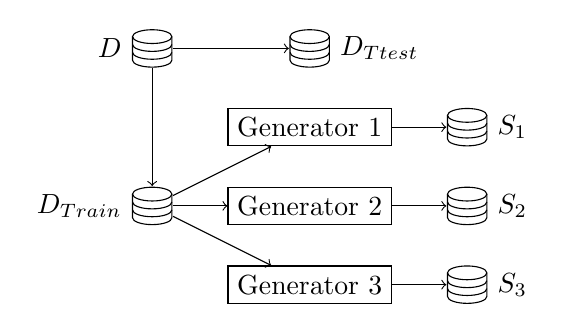
\begin{tikzpicture}
\node[database,label=left:$D$] (d) at (0,0){};
\node[database,label=left:$D_{\text{Train}}$] (train) at (0,-2){};
\node[database,label=right:$D_{\text{Ttest}}$] (test) at (2,0){};

\draw[->] (d) to (train);
\draw[->] (d) to (test);

\def \p {-2} %Bloc position
\def \s {1} %spacing
\node[rectangle,draw] (g1) at (2,\p+\s) {Generator 1};
\node[rectangle,draw] (g2) at (2,\p) {Generator 2};
\node[rectangle,draw] (g3) at (2,\p-\s) {Generator 3};

\draw[->] (train) to (g1);
\draw[->] (train) to (g2);
\draw[->] (train) to (g3);

\node[database,label=right:$S_{1}$] (s1) at (4,\p+\s){};
\node[database,label=right:$S_{2}$] (s2) at (4,\p){};
\node[database,label=right:$S_{3}$] (s3) at (4,\p-\s){};

\draw[->] (g1) to (s1);
\draw[->] (g2) to (s2);
\draw[->] (g3) to (s3);


\end{tikzpicture}
